\chapter[Revisão Sistemática]{Revisão Sistemática}

    Este capítulo apresenta conceitos pertinentes aos principais tópicos que serão abordados
    nesse TCC. Os tópicos abordados são, \textit{Hadoop, MapReduce, Spark, Impala, HBase e
    Cloudera.}

    \section{Hadoop}

        O \textit{Hadoop} foi criado por Doug Cutting, o mesmo criador do \textit{Apache Lucene}, a biblioteca de
        busca textual \cite{white2015}. O Hadoop é composto por dois componentes principais, o HDFS que é um
        sistema de arquivos para ser usado em \textit{cluster}, e o \textit{MapReduce} que é responsável pelo
        processamento dos dados armazenados no sistema de arquivos. O \textit{Hadoop} em comparação com
        outros sistemas de arquivos distribuídos possui é um sistema tolerante a falhas críticas, e foi desenvolvido
        para rodar em máquinas de baixo custo com um modelo de programação simples \cite{alam2014}. Segundo
        \citeonline{alam2014}, o \textit{Hadoop} cobre quase todos os aspectos dos paradigmas de sistemas distribuídos
        como confiabilidade, eficiência, disponibilidade, acurácia e segurança.

        \subsection{Hadoop Distributed File System}

            O HDFS é um sistema de arquivos distribuídos desenvolvido para armazenar arquivos muito grandes
            com um padrão de fluxo de dados, que funcionam dentro de um \textit{cluster} de máquinas de
            baixo custo \cite{white2015}.

            As suas principais características são, lotes de grandes arquivos a serem processados, o fluxo de
            acesso de dados em que o sistema escreve uma vez e lê várias vezes em determinado padrão e
            pôr fim a baixa necessidade de uma estrutura de ponta, pois o próprio sistema já fornece quase
            todos os aspectos dos paradigmas que os sistemas distribuídos tentam cobrir, logo foi desenvolvido
            para rodar em máquinas de baixo custo (computadores domésticos são exemplos de máquinas de
            baixo custo), o sistema se utiliza de implementações contra falhas críticas para, caso um nó venha a
            falhar o HDFS ainda continue trabalhando sem interrupções \cite{white2015}.

            \subsubsection{Bloco de Dados}

                O conceito de bloco de dados, se refere ao contêiner que será utilizado para o armazenamento
                dos dados. Este contêiner possui um tamanho padrão que pode ser definido nas configurações
                do HDFS dependendo da necessidade do cliente. O bloco de dados então é armazenado ao longo
                do \textit{cluster} e suas referências são guardadas.

                O motivo pelo qual se dá preferência a arquivos muito grandes, é pela necessidade de dividir
                esses arquivos em blocos, para que encaixem nos containers. Para \citeonline{white2015},
                ter uma abstração de bloco para um \textit{Distributed File System} (DFS) pode trazer uma série
                de benefícios como o caso de um arquivo ser maior que o disco, então existe a vantagem de ter
                vários discos em \textit{cluster}.

                Outra vantagem, está na abstração dos blocos ao invés de arquivos, e isso simplifica o
                armazenamento. O subsistema de armazenamento usa blocos de dados para simplificar
                o gerenciamento de armazenamento, pois como os blocos possuem tamanhos fixos, fica
                fácil determinar a alocação dos blocos ao longo dos discos \cite{white2015}.

                Não existe necessidade de preocupação com os metadados levando em consideração
                que os blocos são apenas pedaços de dados que são armazenados, os arquivos de
                metadados tais como informações sobre permissões não precisam ser armazenados com
                os blocos, pois existe outro sistema que trata dos metadados separadamente
                \cite{shvachko2010}.

                \begin{figure}[ht!]
                    \centering
                    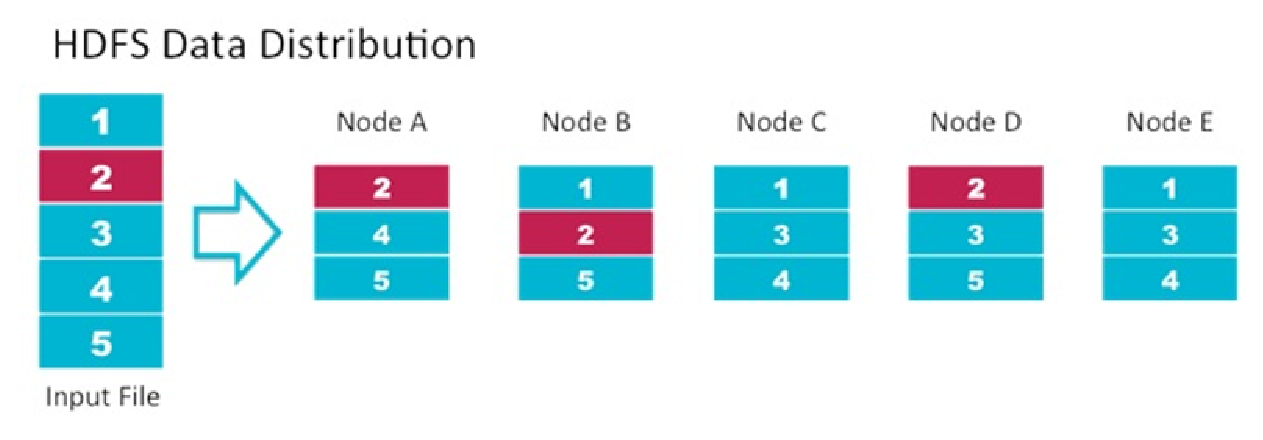
\includegraphics[keepaspectratio=true,scale=0.75]
                        {figuras/figura1.eps}
                    \caption[Distribuição em Blocos no HDFS]{Distribuição em Blocos no HDFS
                    \protect\linebreak Fonte: Colocar a fonte}
                    \label{figura1}
                \end{figure}

                Com a replicação dos dados, temos a garantia de que mesmo que um node venha a falhar o
                dado não será perdido, garantindo a proteção contra falhas críticas e disponibilidade. Essa
                replicação é realizada por padrão de distribuição em até três maquinas, mas essa configuração
                pode ser alterada dependendo da necessidade do cliente para garantir a integridade de seus dados.

            \subsubsection{Arquitetura HDFS}

                Em um cluster de HDFS, existem dois tipos de \textit{nodes} operantes no caso o: \textit{namenode}
                (o mestre) e um certo número de \textit{datanodes} (trabalhadores). O \textit{namenode} gerencia
                o \textit{namespace} e mantêm a arvore do sistema de arquivos e dos metadados para todos os arquivos
                e diretórios na estrutura. Essa informação é armazenada no disco local em forma de dois arquivos, a
                imagem do \textit{namespace} e o log de edição. De acordo com \citeonline{shvachko2010}, o \textit{namenode}
                conhece em quais \textit{datanodes}  determinado arquivo está localizado, porém ele não reconstrói a local,
                por que essa informação é reconstruída dos \textit{datanodes} quando o sistema inicia \cite{white2015}.

                O \textit{client} acessa o sistema de arquivos em nome do usuário, se comunicando com o \textit{namenode}
                e \textit{datanodes}. A interface do cliente é similar ao \textit{Portable Operating System Interface} (sistema
                que o kernel do Linux usa), logo o usuário não precisa saber sobre as funções do \textit{namenode} e
                \textit{datanodes} em específico.

                \begin{figure}[ht!]
                    \centering
                    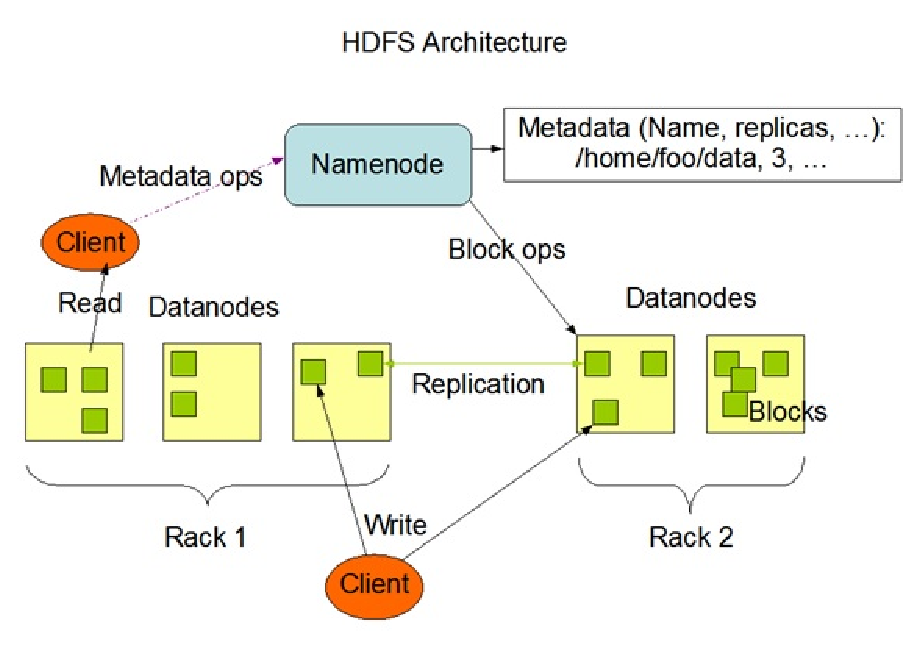
\includegraphics[keepaspectratio=true,scale=0.75]
                        {figuras/figura2.eps}
                    \caption[Arquitetura do HDFS]{Arquitetura do HDFS
                    \protect\linebreak Fonte: Colocar a fonte}
                    \label{figura2}
                \end{figure}

                Na figura \ref{figura2}, temos a visualização da arquitetura do HDFS, o \textit{namenode} manipula
                os metadados que são essenciais para a aplicação \textit{client}, nele temos dados do \textit{namespace}
                e o número de réplicas bem como outras informações a mais, e com o mapeamento desses dados a
                aplicação consegue recuperar o dado que precisa nos \textit{datanodes} referenciados.

            \subsubsection{Processo de Leitura e Escrita}

                Quando uma aplicação vai ler um arquivo, o HDFS \textit{client} pergunta ao \textit{namenode} pela
                lista de \textit{datanodes} que guardam as réplicas de determinado bloco do arquivo. Só então a
                aplicação comunica-se com o \textit{datanode} diretamente e requisita a transferência de determinado
                bloco. É possível visualizar esse processo de forma detalhada na figura \ref{figura3}, o qual temos uma aplicação do
                HDFS em cima de uma \textit{Java Virtual Machine} (JVM) que se comunica com os \textit{nodes} em
                determinada ordem, para obter um determinado arquivo \cite{shvachko2010}.

                Já quando a aplicação escreve, ele pergunta ao \textit{namenode} para que escolha os \textit{datanodes}
                que serão utilizado para armazenar o primeiro bloco do arquivo, então o \textit{client} organiza uma
                \textit{pipeline} de \textit{node} para \textit{node} e envia os dados. Quando o primeiro bloco é
                preenchido, o \textit{client} faz uma nova requisição por novos \textit{datanodes} a serem escolhidos
                para guardarem as réplicas do próximo bloco. Esse mesmo processo é possível de ser visualizado na figura
                \ref{figura4} com detalhes \cite{shvachko2010}.

                \begin{figure}[ht!]
                    \centering
                    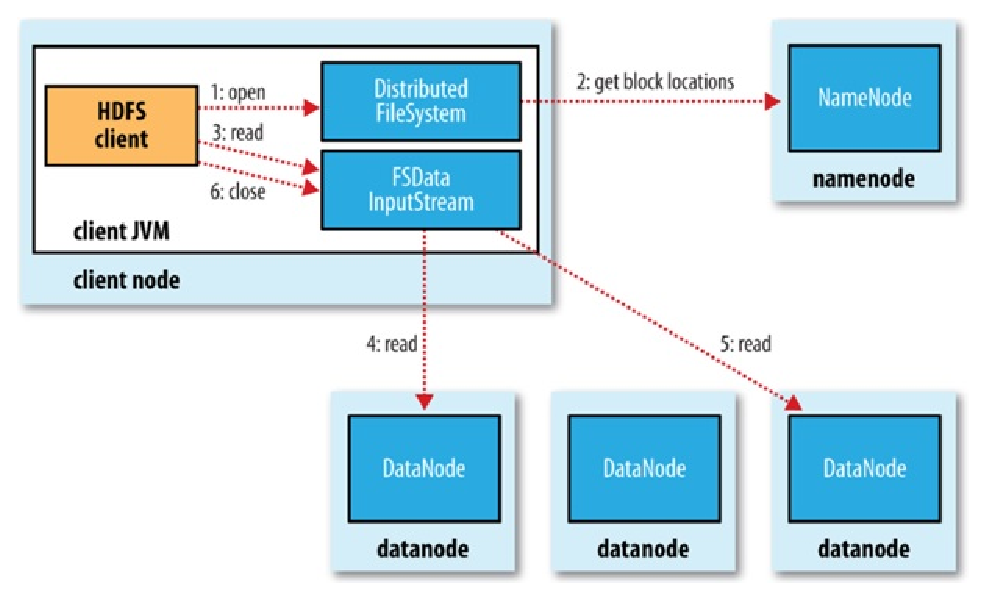
\includegraphics[keepaspectratio=true,scale=0.75]
                        {figuras/figura3.eps}
                    \caption[Processo de Leitura no HDFS]{Processo de Leitura no HDFS
                    \protect\linebreak Fonte: \citeonline{white2015}}
                    \label{figura3}
                \end{figure}

                \begin{figure}[ht!]
                    \centering
                    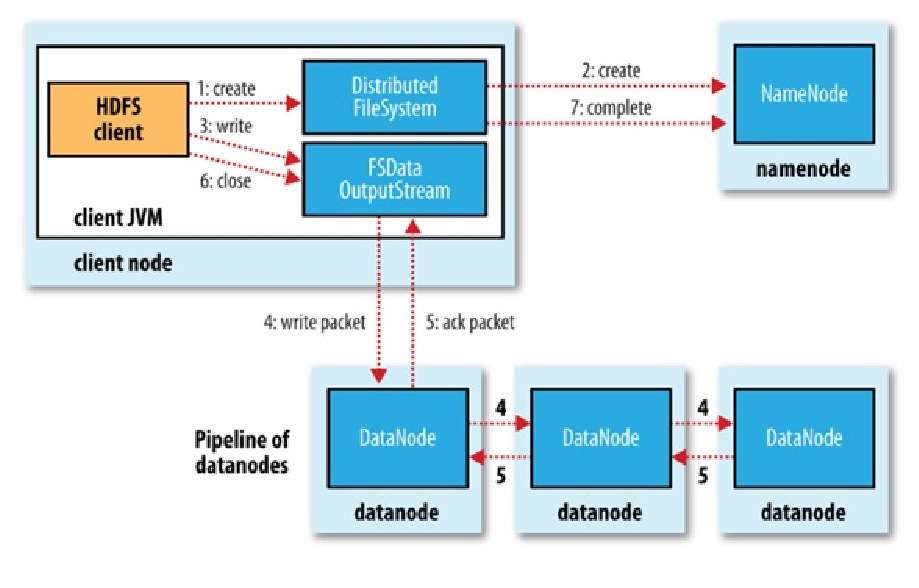
\includegraphics[keepaspectratio=true,scale=0.75]
                        {figuras/figura4.eps}
                    \caption[Processo de Escrita no HDFS]{Processo de Escrita no HDFS
                    \protect\linebreak Fonte: \citeonline{white2015}}
                    \label{figura4}
                \end{figure}

        \subsection{Map Reduce}

            O desenvolvimento do \textit{MapReduce} surgiu de uma necessidade de processamento de uma grande
            quantidade de dados brutos, com o objetivo  de computar diversos tipos de dados derivados, como índices,
            representações gráficas acerca de determinados dados, sumarização, dentre outras \textit{queries} frequentes
            usadas no dia-a-dia. Porém os dados de entrada são geralmente grandes e computacionalmente precisam ser
            distribuídos ao longo de milhares de máquinas, para que seja possível de terminar em uma quantidade de
            tempo razoável \cite{dean2008}.

            De acordo com \citeonline{dean2008}, o \textit{MapReduce} foi desenvolvido em resposta a complexidade
            que se tem para processamento de dados em lote em uma arquitetura distribuída. Então essa camada de
            abstração permite expressar uma computação mais simples, mas que por baixo, abstrai detalhes de computação
            paralela, tolerância a falhas, distribuição de dados e balanceamento de carga só que em uma biblioteca.

            O \textit{MapReduce} funciona quebrando o processo em duas fases, a fase de mapeamento e a fase de
            redução. Cada fase tem um par de chave-valor como entrada e saída. O programador também especifica
            as duas funções, a função de mapeamento e a função de redução \cite{white2015}.

            A função de mapeamento escrita pelo usuário, precisa de um par na entrada e produz um intervalo de pares
            de chave-valor. A biblioteca agrupa juntamente com todos os valores intermediários associados com a
            mesma chave intermediária e repassa para a função de redução. Já a função de redução aceita uma
            chave intermediária e um intervalor de valores para aquela chave. Esses valores são fundidos para
            forma um intervalo menor ainda de valores, tipicamente apenas zero ou uma entrada de valor é produzido
            por invocação de redução. Esses valores intermediários são produzidos pelas funções de redução do
            usuário via \textit{iterator}. Isto nos permite manejar a lista de valores que são muito grandes para
            caber na memória \cite{dean2008}.

            De acordo com \citeonline{white2015} o \textit{MapReduce job} é uma unidade de trabalho que a aplicação
            deseja que seja processada, e consiste em uma entrada de dados, a definição do \textit{MapReduce} programado
            e a configuração das informações. O Hadoop executa o \textit{job} dividindo ele em tarefas de dois tipos, as
            chamadas tarefas de mapeamento e tarefas de redução. Essas tarefas são organizadas usando o YARN (Yet
            Another Resource Negotiator) e são executadas nos \textit{nodes} do cluster, e se a tarefa falha, ela será
            automaticamente reorganizada para a fila de execução em um \textit{node} diferente. Na figura \ref{figura5}
            temos a ilustração no processo \textit{shuffle} e {sort} que é um processo que garante que toda entrada para
            cada redutor tenha uma chave, e que transfira os valores da saída do mapeamento para a entradas dos
            redutores \cite{white2015}.

            \begin{figure}[ht!]
                    \centering
                    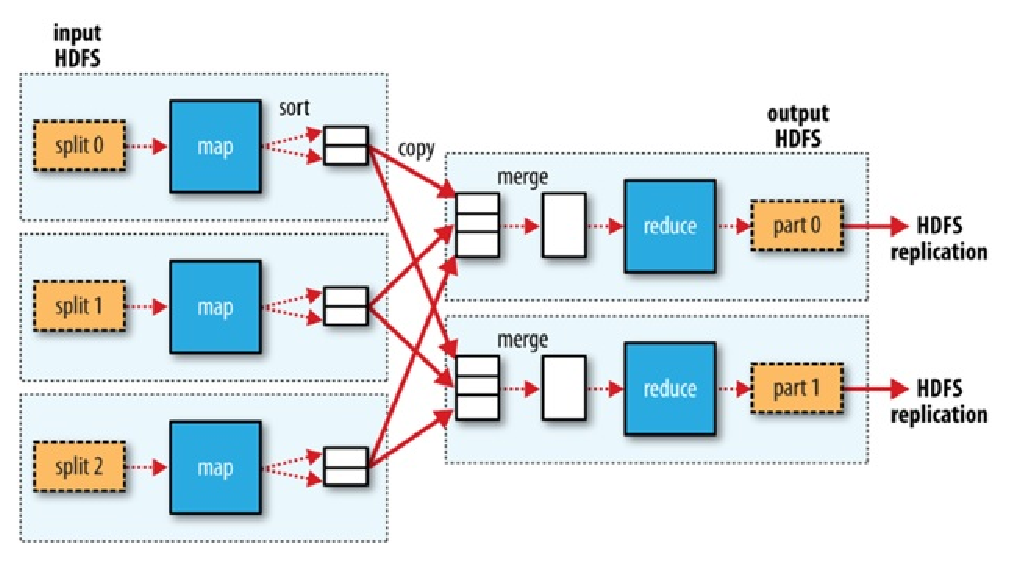
\includegraphics[keepaspectratio=true,scale=0.75]
                        {figuras/figura5.eps}
                    \caption[Fluxo de dados em um \textit{MapReduce} com múltiplas tarefas de redução]
                    {Fluxo de dados em um \textit{MapReduce} com múltiplas tarefas de redução
                    \protect \linebreak Fonte: \citeonline{white2015}}
                    \label{figura5}
            \end{figure}

            \subsubsection{Arquitetura do MapReduce}


        \subsection{YARN}


    \section{HBase}

    \section{Spark}

    \section{Impala}



